% !TeX program = xelatex
\documentclass{alex_bericht}
\usepackage[export]{adjustbox}

\def\NFe{N_{\text{Fe}}}
\def\NH{N_{\text{H}}}

\begin{document}
%Seiten ohne Kopf- und Fußzeile sowie Seitenzahl
\pagenumbering{Roman}
\def\settitle{Sun spectroscopy}
% !TeX root = Bericht.tex
% !TeX spellcheck = de_DE
\thispagestyle{empty}
\titlehead{
\includegraphics[width=5cm]{logo.jpg}}
\title{\settitle}
\author{Alexander Helbok\thanks{\href{mailto:alexander.helbok@student.uibk.ac.at}{alexander.helbok@student.uibk.ac.at}},
		Jakob Höck \thanks{\href{mailto:jakob.hoeck@student.uibk.ac.at}{jakob.hoeck@student.uibk.ac.at}},
		Max Koppelstätter\thanks{\href{mailto:max.koppelstaetter@student.uibk.ac.at}{max.koppelstaetter@student.uibk.ac.at}}}
\date{\today}
\maketitle
\vfill 


\section*{Abstract}
This experiment deals with taking an astrophysical spectrum of the sun. Thereby, some corrections of the raw data have to be carried out. A bias subtraction and a flatfield correction are accomplished, in addition to a calibration with ThAr-lamps. After these corrections, Fe I lines of the sun's spectrum are analysed, to determine the curve of growth. Using a fit, the effictive temperature of the sun can be determined as \SI{5521(110)}{K} and the abundance of Iron relative to hydrogen as 0.043(7) \%. 
\vspace{1.5cm}


%Inhaltsverzeichnis
{\hypersetup{linkcolor=black}
\clearpage
\tableofcontents

%Verzeichnis aller Bilder
%\listoffigures

%Verzeichnis aller Tabellen
%\listoftables}
\cleardoubleoddpage

\pagenumbering{arabic}
% !TeX root = Bericht.tex
% !TeX spellcheck = en_US
\section{Introduction}

Without lasers, the world would look quite different from the world we know. From GPS to accurate clocks, lasers are omnipresent in the modern world, essential in a big variety of applications. 
But not only technical applications are worth mentioning here; they also play an indispensable
role in various physical experiments, shedding light on phenomena ranging from quantum mechanics to material science. In this experiment, we created setups, in which lasers are combined with an electro-optical-modulator (EOM). This component contains a crystal, which changes its optical properties when exposed to an electric field. This behaviour is called the electro-optical effect, which can be applied in many ways. For example, one can create lenses with adaptive focal length as well as optical switches. In the first setup, a Mach-Zehnder-interferometer is set up, with an EOM placed in one of its arms. The interference pattern of the output beam is recorded by a photodiode, enabling us to determine the half wave voltage and the bandwidth. Afterwards, an optical switch is realized in a simpler setup, where a laser beam passes an EOM and finally enters a photodiode. Before and after the EOM, waveplates and polarizers are used to inspect the behavior of different polarisation's of the laser light. 

The first chapter of this report deals with the necessary theory, followed by the experimental setup and procedure. In the next chapter, the results and data analysis are presented. Finally, the results are interpreted. 

% !TeX root = Bericht.tex
% !TeX spellcheck = de_DE
\section{Theory}
\label{sec:theorie}
In this section, all necessary theoretical backgrounds are presented. Some theory belonging to spectroscopy is described as well as corrections of raw data frames.
\subsection{Spectroscopy}


When analysing absorption lines in a spectrum, the equivalent width of a line is determined. This width $EW$ is formally defined as 
\begin{equation}
	EW=\int \frac{I_0-I_\lambda}{I_0}d\lambda,
\end{equation}
where $I_0$ is the constant continuum intensity, and $I_\lambda$ is is the intensity measured at a certain wavelength $\lambda$. Graphically, the equivalent width can be described as the width of a square with length of the continuum intensity, as can be seen in \autoref{bild_linewidth}. The area of the square hereby has to equal the missing area of the absorption line. 

\begin{figure}[H]
	\centering
	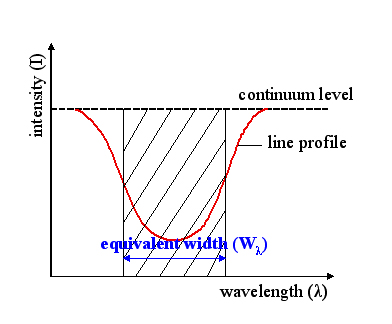
\includegraphics[width=0.5\textwidth]{Definition_of_equivalent_width}
	\caption{Visualization of the equivalent width of a line profile of an absorption line. Figure taken from \cite{bild_linewidth} }
	\label{bild_linewidth}
\end{figure}
The equivalent width depends on the number of atoms $N_i$ in an absorbing medium. The number of atoms $N_i$ is relative to a gas column with a certain volume. The behavior of the equivalent width dependent on $N_i$ is called the curve of growth. Atomic states are distributed via Boltzmann-distribution, leading to
\begin{equation}
	EW_\lambda=\frac{N_{r0}}{g_{r0}}g_{rs}f_{rs}\lambda^2 \exp{(-\chi_i/(k_{\mathrm{B}}T)}. \label{schwierig}
\end{equation}
Here, $f$ describes the oscillator strengths, $g$ the degeneracy, $r$ and $s$ are the quantum numbers of both levels involved in the transition. This approximation, however, is only valid for thin absorbing layers. Above the validity range of the approximation, saturation occurs. Doppler and Stark broadening are getting relevant here, and lead the curve of growth to a new regime \cite{spectroscopy}.
Based on \autoref{schwierig}, we can derive 
\begin{equation}\label{eqn:line}
	\log(EW_\lambda/\lambda)-\log(\lambda g f)=-\frac{5040}{T}\chi+\log(N_\mathrm{i}/N_\mathrm{H}). 
\end{equation}
Using this relation, the growth curve can be determined, using the equivalent width, wavelength and the factor $\log{(gf)}$. To receive this data, we are fitting a gaussian function to every peak. Out of the fit-parameters, we get the equivalent width and wavelength, the third factor is used from a table. 
\subsection{Echelle-spectrograph}
In order to get a spectrum out of light, we need to disperse the light. Therefore, in our case, an Echelle-spectrograph is used. This type of spectrograph offers high resolutions, meaning that it can resolve a large range of wavelengths. The intensity, in contrast, is very low for high resolutions, as the intensity is distributed on many orders, in contrast to focusing on only one specific order. 
A second grating with lower resolution is used after the first one, and disperses light perpendicular. Because of this setup, the spectra of individual orders are placed on top of each other in the resulting frame. As a result of the two gratings, the recorded spectra are curved, due to occuring nonlinear dispersion terms. 



%\begin{figure}[H]
%    \centering
%    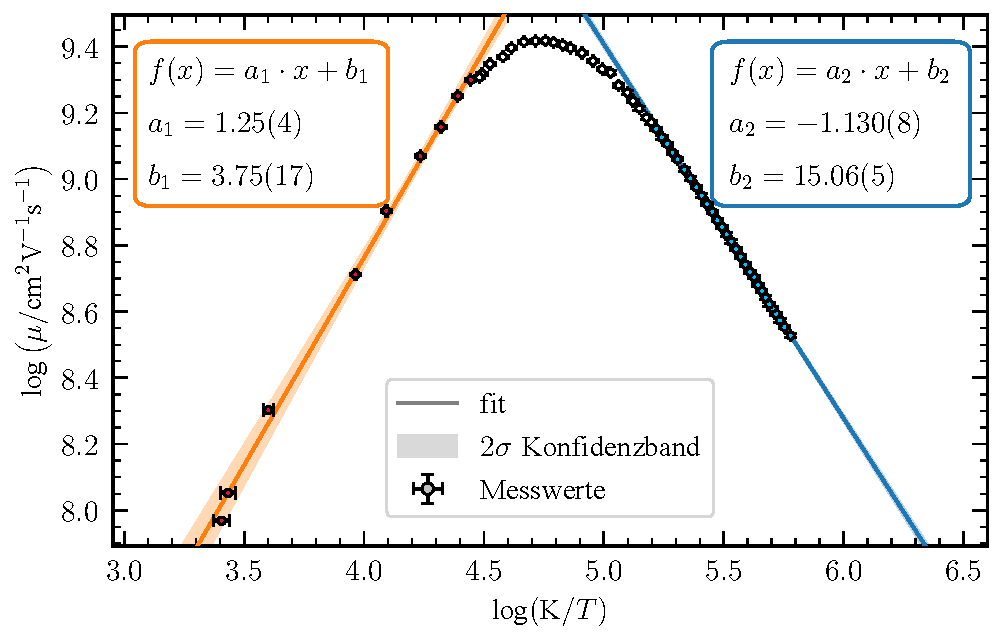
\includegraphics[width=\textwidth]{plot3.pdf}
%    \caption{}
%    \label{fig:plot3}
%\end{figure}


\subsection{Data processing}
In order to get a sun spectra of high quality, we need to process the raw data. Therefore, some important measurements and corrections have to be made. 
The first one of these is called the bias subtraction. It gets rid of signal that is recorded, while the sensor is not exposed to any light. Thus, the bias is a constant offset, which has to be subtracted from the raw file. The bias can be measured by taking pictures without exposing the CCD sensor to light. \newline

The second step is to do a flatfield correction. The CCD sensors sensitivity is not equal on the complete sensor. Therefore, the whole sensor is exposed uniformly to a light source, the sensors response then should be constant for a perfect sensor. Nevertheless, some deviations can be seen in these flatfield frames. To correct the raw data, the data frame has to be divided by an averaged flatfield frame.  \newline

As it is unknown which pixel on the CCD corresponds to which wavelength, a wavelength calibration needs to be carried out. To do so, the sensor is illuminated with a ThAr-lamp. The emitted wavelengths of this lamp is known, thus the pixels can be calibrated this way. 

After these three steps of correcting and calibrating, the two-dimensional frame needs to be converted to a one-dimensional spectrum. 


%
% !TeX root = Bericht.tex
% !TeX spellcheck = en_US
\section{Experimental setup and procedure}\label{sec:procedure}
The experiments begin with a characterization of the Gaussian beam. Afterward, modes of the laser in a cavity are analyzed. 

\subsection{Beam profiling}
The first step is to determine the width of the waist of the beam emitted by a HeNe laser with a wavelength of \( \lambda = 633 \unit{nm} \). After the laser, a Faraday isolator (FI) is placed, which protects the laser from back reflections.

The beam width is measured at various distances from the laser. In total 11 measurements are taken in steps of \SI{1.5}{cm}, starting closely after the FI. The beam width was measured using a waistmeter, which contatins a photodiode measuring the intensity, and a rotating disc. This rotating disc alternately covers the photodiode so that the width of the beam can be determined if the disc's rotation speed and geometry are known. Since the waistmeter indicates the actual diameter, it must later be halved to obtain the radius of the beam.

After these measurements, a lens with a focal length of $f = 100 \unit{mm}$ is placed after the Faraday isolator. The same procedure is then repeated.

\subsection{Mode matching}
\label{subsec:mode}
In preparation for the experiment, the beam waist of the cavity was determined. This can be done using \autoref{eqn:w0} and $r = L = 150 \unit{mm}$ and we get $w_0 = 122.93 \unit{\micro\m}$. 

The next step is to match the resonator waist to the beam waist of the laser using a suitable lens. In \autoref{lens_simulation} the simulated beam with a lens is shown, which is used to determine the best focal length of the lens we want to use for the following steps. In the simulation, the result for the beam diameter and the divergence angle from the first part of the experiment is used. 

\begin{figure}[H]
	\centering
	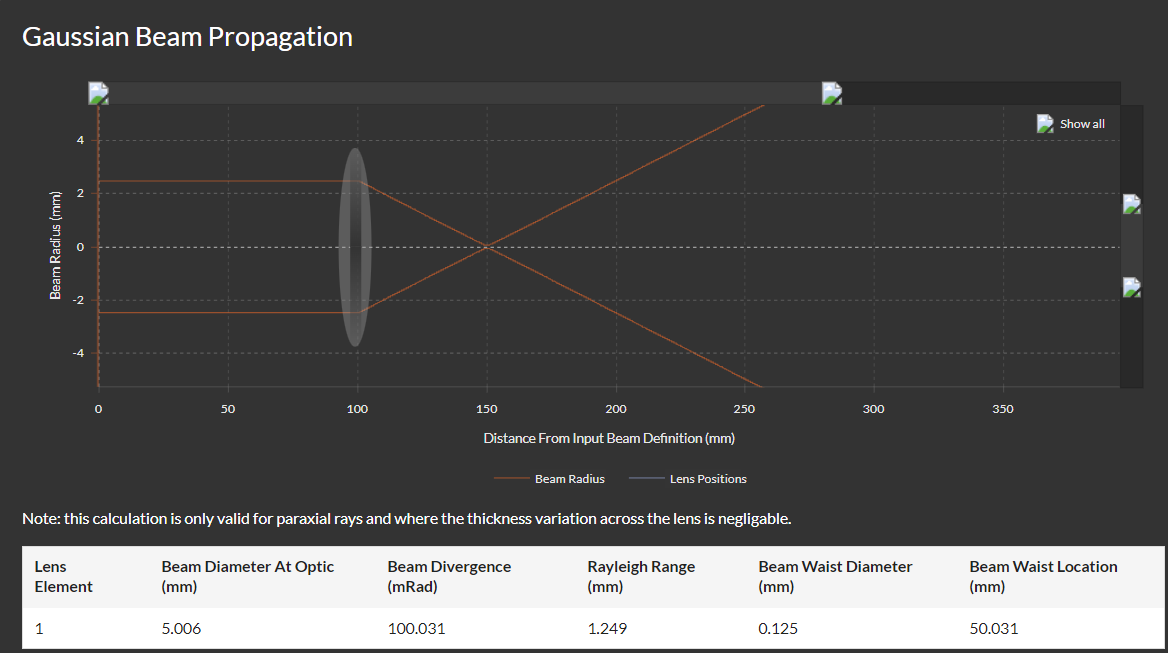
\includegraphics[width=\textwidth]{simulation_lens}
	\caption{Simulation for a Gaussian beam with a beam waist diameter of \SI{0.44}{mm} and a full angle beam divergence of \SI{1.83}{mRad}, including a lens with focal length \SI{200}{mm}, placed at \SI{550}{mm} from the beam focus. Simulation made with \cite{lightmachinery}.} 
	\label{lens_simulation}
\end{figure}

It turns out that \SI{200}{mm} yields the results. Once the lens is in place, the next step is to align it correctly, then adjust the subsequent mirrors and the cavity mirrors to ensure that the laser beam is in a straight line. This entire structure can be seen in \autoref{fig:Gesamtaufbau}. 

\begin{figure}[H]
	\centering
	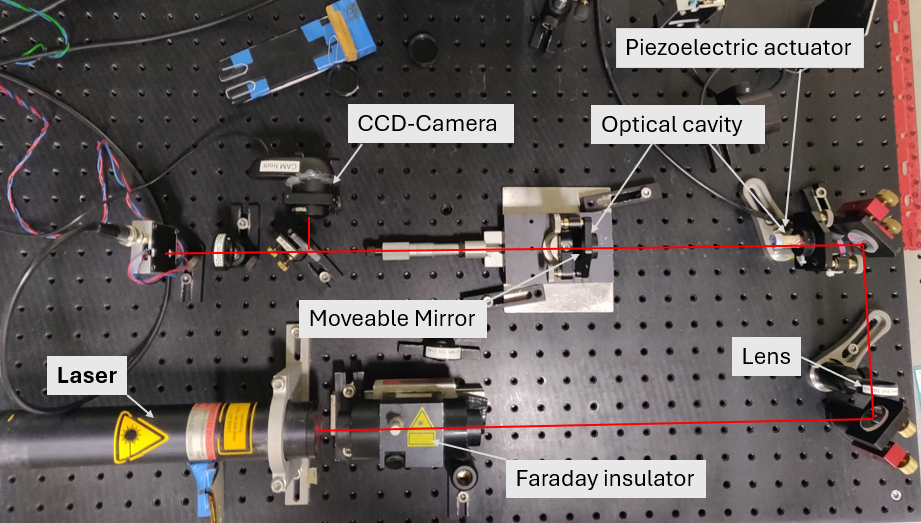
\includegraphics[width=\linewidth]{AufbauBild}
	\caption{The entire setup from the laser to the photodiode and the CCD camera is visible via the Faraday isolator, built-in lens, and optical cavity, which includes a piezoelectric actuator and an adjustable mirror. A beam splitter allows simultaneous irradiation of the two objects. The Faraday isolator ensures that the reflected beam does not return to the laser.}
	\label{fig:Gesamtaufbau}
\end{figure}

After the laser beam leaves the Faraday isolator it passes through a lens and is redirected by two mirrors. It then enters a cavity consisting of two mirrors, one of which is placed on a movable mount, whilst the other is mounted onto a Piezo-transducer, connected to a function generator. This enables us to minimally change the cavities length, effectively scanning frequencies. After the latter cavity mirror, the laser beam passes a beam splitter, directing one part onto a CCD-camera, which is used to take pictures of the incoming beam, while the other part is directed onto a photodiode, connected to an oscilloscope.

\subsection{Study of cavity modes}
\label{subsec:CavityModes}
The resonator is first visually aligned by overlapping the mirror reflections and then fine tuned using the output on the oscilloscope maximizing the transmission of the TEM$_{00}$ mode. Here we recorded two spectra, one with perfect alignment to study the transmission and the other one with slightly misaligned mirrors to measure the distance to half axial modes.

After this, the length of the resonator was increased by \( 13.53(1) \unit{mm} \) using the adjustable mirror to make higher modes visible. In a confocal resonator, these are always projected between two intensity peaks (see \autoref{subsec:OptRes}). One of the deflection mirrors was then adjusted so that the laser no longer falls directly into the resonator. This allows higher modes to be detected on the photodiode, as well as the CCD camera. It is important to note that any change in resonator or laser alignment can affect the visible modes, so careful calibration and control is required throughout the process. The oscilloscope readings and images from the CCD camera are stored for later analysis.

%
% !TeX root = Bericht.tex
% !TeX spellcheck = de_DE
\section{Ergebnisse}
Im gesamten Versuch wurde die Strahlungsintensität in Abhängigkeit von diversen Parametern untersucht. Die Intensität lässt sich dabei über ein Geiger-Müller Zählrohr (GMZ) ermitteln, welches Ionisierungsereignisse \( N \) misst. Diese folgen der Poisson Statistik, weshalb der Fehler auf \( \delta N = \sqrt{N} \) gesetzt wurde. Diverse Parameter des GMZ und der Röntgenquelle können über eine Software eingestellt werden und werden als Fehlerfrei angenommen. 

Bevor wir mit dem GMZ das Absorptionsverhalten diverser Materialien untersuchen, wollen wir dieses noch charakterisieren. Dafür wurde das Zählrohr auf \ang{5.5} geneigt, um eine Sättigung durch direktes Einstrahlen zu verhindern, und die Spannung von \( 300 \unit{V} \) bis \( 500 \unit{V} \) erhöht. Dabei wurden die Schritte so gewählt, dass Bereiche mit einer großen Änderung von \( N \) besser aufgelöst sind. Für jede Spannung wurden drei Werte händisch notiert, über die wir dann mitteln. Der Poisson Fehler wird dann nach der Mittlung angewendet. In \autoref{fig:Ex1} sind die gemessenen Zählraten $N$ auf die Zählrohrspannung $U$ aufgetragen. Zusätzlich wurde eine Exponentialfunktion an die rot markierten Datenpunkte gefittet, da diese optisch passt und sich Werte, wie Betriebsspannung, leicht ermitteln lassen.

\begin{figure}[H]
	\centering
	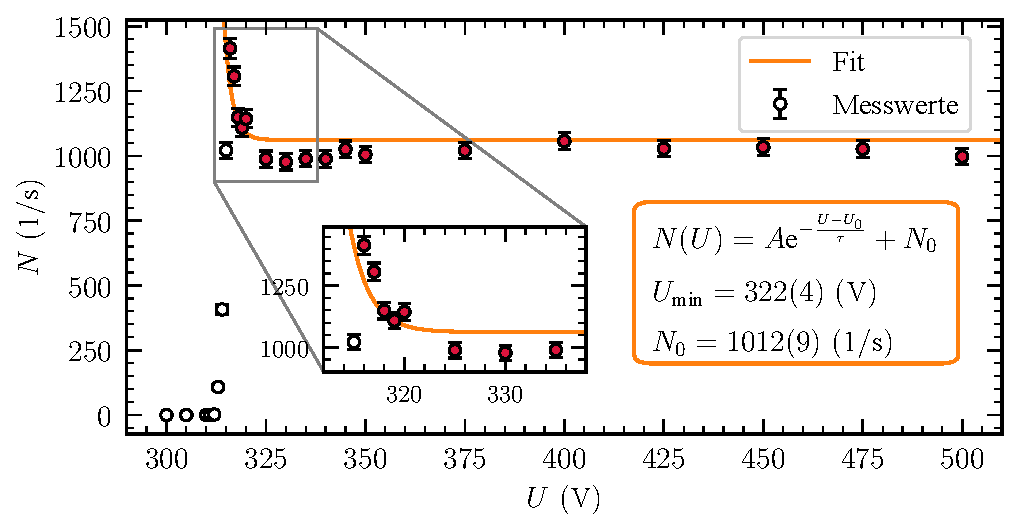
\includegraphics[width=\textwidth]{Ex1}
	\caption{Die gemessene Zählrate \( N \) ist auf die Wellenlänge \( \lambda \) aufgetragen. Die Daten sind mit poissonschem \( 1\sigma \) Unsicherheit angegeben. An rot markierte Datenpunkte wurde eine Exponentialfunktion angepasst, um die Betriebsspannung zu bestimmen. Die ermittelten Werte sind in der Ecke rechts unten zu sehen.}
	\label{fig:Ex1}
\end{figure}

In \autoref{fig:Ex1} lässt sich die Zählrohrcharakteristik des GMZ gut erkennen. Zählereignisse finden zunächst aufgrund zu geringer Spannung nicht statt, nehmen dann schnell zu und pendeln sich dann zu einen konstanten Wert ein. Die untere Grenze des Plateaubereichs wurde da gesetzt, wo die angepasste Exponentialfunktion nur mehr \( 1\% \) über dem konstanten Offset \( N_0 \) liegt (\( U_{\text{min}} = U_0 + \tau\log\left( A/0.01N_0 \right) = 322(4) \unit{V} \)). Der Überschuss der Zählereignisse vor dem Plateau wird wahrscheinlich durch Mehrfachzählung eines Ionisierungsereignisses verursacht. 

Jetzt wo der Arbeitsbereich des GMZ bekannt ist, wird dieser für die restlichen Messungen auf \( 500 \unit{V} \) gesetzt. Das kontinuierliche Röntgenspektrum lässt sich durch Einführen eines \ch{LiF} Kristalls mit Gitterebenenabstand \( d = 201 \unit{pm} \) ausmessen. Dabei wird der Winkel zwischen Kristallebene (an welcher Reflexion stattfindet) und GMZ von \ang{5.5} bis \ang{35} in \ang{0.1} Schritten verändert. Dabei wird das kontinuierliche Spektrum für festen Winkel dank der Bragg Reflexion nach einzelnen Wellenlängen gefiltert (siehe \autoref{bragg_schema}). In \autoref{fig:Ex2} ist das gemessene Spektrum auf die Wellenlänge, sowie Energie aufgetragen.

\begin{figure}[H]
	\centering
	\adjincludegraphics[width=\textwidth, clip, trim = {0 {.15\height} 0 {.15\height}}]{Ex2}
	\caption{Die gemessene Zählrate \( N \) ist auf die Wellenlänge \( \lambda \) aufgetragen. Die Energie der Photonen lässt sich aus der Wellenlänge bestimmen und ist als zweite x-Achse an der oberen Kante zu sehen. Die Daten sind mit poissonschem \( 1\sigma \) Unsicherheit angegeben, wobei diese zu klein ist um ausgemacht werden zu können. An die Daten wurde in orange eine Kombination aus drei Lorentz und einer linearen Funktion angepasst. Aus dem Fit lässt sich die Position der Peaks bestimmen, was links neben dem jeweiligen Peak vorgemerkt ist.}
	\label{fig:Ex2}
\end{figure}

Man kann in \autoref{fig:Ex2} einen kontinuierlichen Hintergrund mit drei prominenten Peaks erkennen. Letztere stammen von K Übergängen in der Anode. %(see \autoref{}).
Um die Energie der atomaren Übergänge zu bestimmen, wurde eine Multilorentz Funktion an die Daten angepasst und ist in orange zu sehen. Diese besteht aus der Summe von drei unabhängigen Lorentz Funktionen, auf welche ein konstanter Hintergrund addiert wurde. Aus dem Fit lassen sich Übergangsenergien zu
\begin{equation*}
	E_1 = 8.41(7) \unit{keV} \qquad E_2 = 9.7(2) \unit{keV} \qquad E_3 = 11.4(2) \unit{keV}
\end{equation*}
bestimmen, wobei als Fehler die Halbwertsbreite der Lorentz-Funktionen gewählt wurde. Die Literaturwerte für die Energie der Peaks betragen \autocite{SpektrumWolfram}
\begin{equation*}
	E_{L_{\alpha 1}} = 8.39 \unit{keV} \qquad E_{L_{\beta 1}} = 9.67 \unit{keV} \qquad E_{L_{\gamma 1}} = 11.28(2) \unit{keV} \qquad E_{L_{\gamma 2}} = 11.6 \unit{keV} 
\end{equation*}
Dabei ist $E_1$ dem Literaturwert $E_{L_{\alpha 1}}$,  $E_2$ dem Literaturwert $ E_{L_{\beta 1}}$ und $E_3$ den Literaturwerten $E_{L_{\gamma 1}}$ und $E_{L_{\gamma 2}}$ zuzuordnen. Für die letzen beiden ist die Auflösung der Messung leider nicht groß genug, um einen sinnvollen Fit zuerstellen, gleiches gilt für den $L_L$ Übergang. Zu erkennen sind diese jedoch klar in \autoref{fig:Ex2}.

Die Maximalenergie (und somit minimale Wellenlänge) der Röntgenphotonen hängt nur von der Beschleunigungsspannung \( U \) und der Elementarladung \( e \) ab. Misst man nun \( \lambda_{\mathrm{min}} \) für mehrere Werte von \( U \), kann man über einen passenden Fit den Wert einer Naturkonstante aus \autoref{eq:Plank} ermitteln. Dafür wurde die Spannung von \( 15 \unit{kV} \) bis \( 30 \unit{kV} \) in \( 2.5 \unit{kV} \) Schritten erhöht. Für jede Spannung wurde \( \lambda_{\mathrm{min}} \) folgendermaßen berechnet: das Spektrum wurde in Schritten von \ang{0.1} aufgenommen, wobei das Messintervall vorab manuell abgeschätzt wurde. Aus den ersten \( 10 \) Datenpunkten wurde der Mittelwert und die Standardabweichung der vorhandenen Hintergrundstrahlung abgeschätzt. Das Röntgensignal wurde als registriert angesehen, sobald der erste Datenpunkt mehr als \( 3\sigma \) vom Mittelwert abweicht, da die Wahrscheinlichkeit, dass dies durch Zufall eintrifft klein genug ist (0.3\%). \( \lambda_{\mathrm{min}} \) liegt dann in der Mitte zwischen dem ersten Datenpunkt des Röntgensignals und dem davor, mit der halben Breite des Intervalls als Unsicherheit. Dieser Prozess ist in \autoref{fig:Ex3} links dargestellt, während rechts die ermittelten \( \lambda_{\mathrm{min}} \) auf die Beschleunigungsspannung \( U \) aufgetragen ist. Zudem ist in orange eine Funktion gefittet.

\begin{figure}[H]
	\centering
	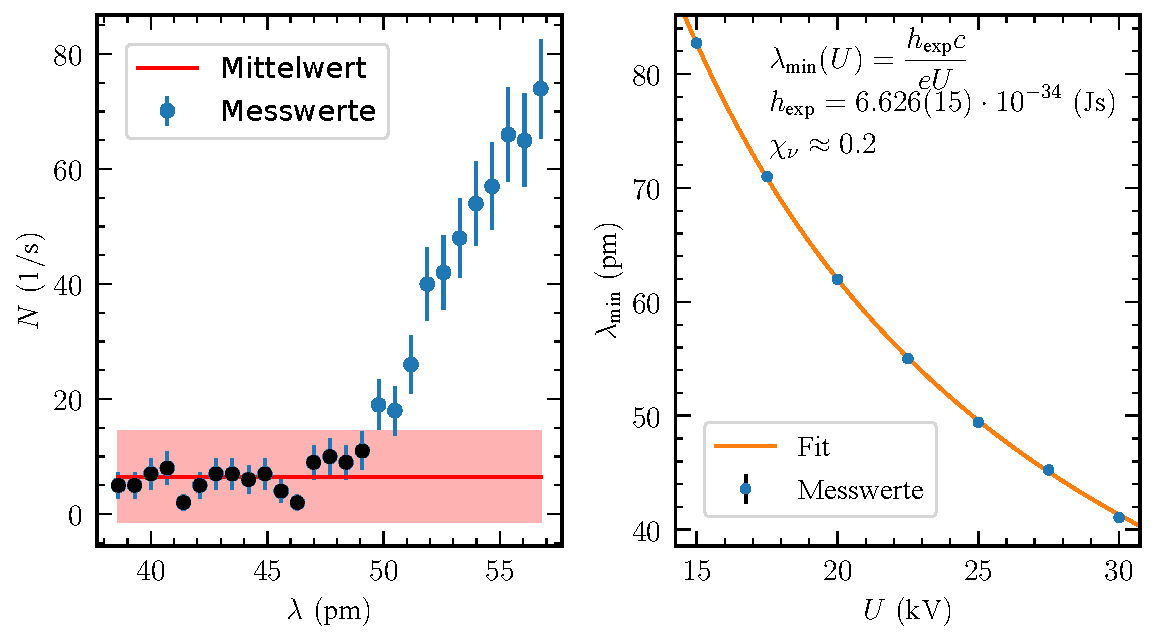
\includegraphics[width=\textwidth]{Ex3}
	\caption{\textbf{Links} ist exemplarisch die Bestimmung von \( \lambda_{\text{min}} \) dargestellt. Dabei wurde der Mittelwert der Daten im konstanten Bereich (Datenpunkte sind rot markiert) berechnet und mit einem \( 3\sigma \) Fehlerband bestückt. \( \lambda_{\text{min}} \) liegt dann in der Mitte zwischen dem ersten Wert, welcher mehr als \( 3\sigma \) vom Mittelwert abweicht, und dem davor. \textbf{Rechts} ist \( \lambda_{\text{min}} \) auf die gesetzte Beschleunigungsspannung \( U \) aufgetragen. In orange wurde eine Funktion an alle Datenpunkte angepasst, aus welcher sich die Planck Konstante ermitteln lässt. Die \( 1\sigma \) Fehler sind nicht sichtbar, da sie zu klein sind.}
	\label{fig:Ex3}
\end{figure}

Im rechten Plot in \autoref{fig:Ex3} sieht man, dass die ermittelten \( \lambda_{\mathrm{min}} \) gut zur Theorie passen. Die Fehler von \( \lambda_{\mathrm{min}} \) wurden sogar etwas zu groß abgeschätzt, was sich im reduzierten Chi-Quadrat \( \chi_\nu \approx 0.2 \) widerspiegelt (sollte bei 1 liegen). Vergleicht man den gefitteten Wert der Planck Konstante mit dem Codata Referenzwert \autocite{codata}
\begin{equation*}
	h_{\text{exp}} = 6.626(15) \cdot 10^{-34} \unit{Js} \qquad\text{und}\qquad h_{\text{lit}} = 6.626 \cdot 10^{-34} \unit{Js},
\end{equation*}
dann treffen wir dieses im Rahmen unserer Unsicherheit.

Weiters können wir noch den Einfluss von diversen Materialien auf die Intensität der Röntgenstrahlung untersuchen. Dafür wurde Zink und Aluminium in unterschiedlichen Dicken vor den GMZ eingeführt und die Zählrate gemessen. In \autoref{fig:Ex4_1} sind die Daten dargestellt, wobei der Datenpunkt bei \( d = 0 \unit{mm} \) verwendet wurde, um die restlichen Messwerte zu normalisieren und untereinander vergleichbarer zu machen. Der erste Datenpunkt hat dann per Definition keine Unsicherheit mehr; diese fließt in die Unsicherheit der restlichen Werte ein. Die Messungen wurden bei \( \lambda = 73.4 \unit{pm} \) (blau in \autoref{fig:Ex4_1}) und \( \lambda = 104.3 \unit{pm} \) (orange) durchgeführt. Zusätzlich wurden Exponentialfunktionen der Form \( N(d)/N_0 = \exp(-\mu d) + c \) angepasst, mit dem Absorptionskoeffizienten \( \mu \) und der Hintergrundstrahlung \( c \) als freie Parameter.

\begin{figure}[H]
	\centering
	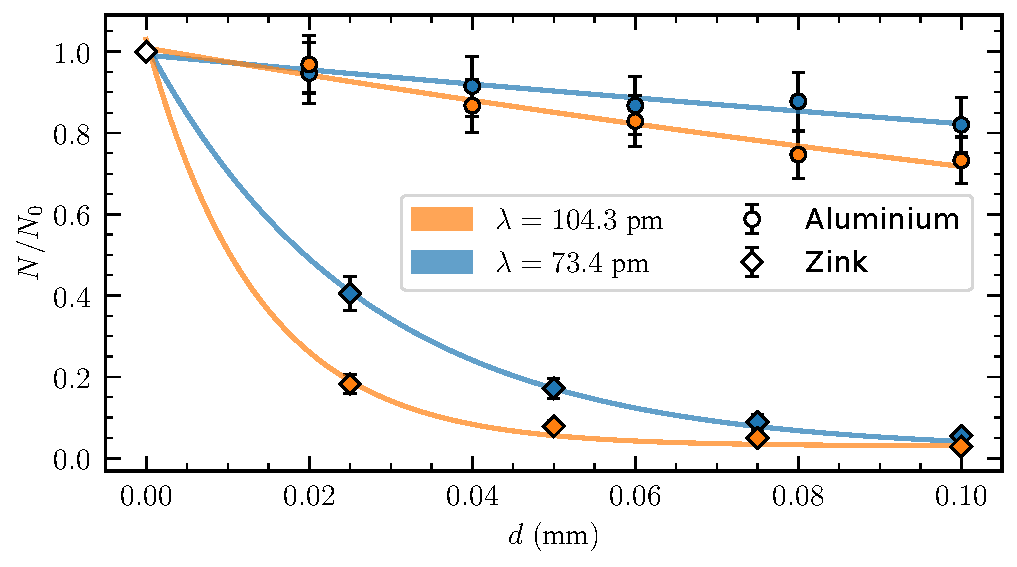
\includegraphics[width=\textwidth]{Ex4_1}
	\caption{Die Zählrate mit Absorber wurde mit der Rate ohne Absorber normalisiert \( N/N_0 \) und auf die Dicke \( d \) des Absorbers aufgetragen. Der Datenpunkt bei \( d = 0 \unit{mm} \) ist somit der Referenzwert für alle Messungen und wird ohne Fehler angegeben. Zwischen den zwei untersuchten Materialien kann man anhand der marker der Datenpunkte unterscheiden, während Messungen verschiedener Wellenlängen farblich auseinanderzuhalten sind. Zudem wurden Exponentialfunktionen der Form \( N/N_0(d) = \exp(-\mu d)+c \) angepasst und als durchgezogene Linie in der Graphik dargestellt.}
	\label{fig:Ex4_1}
\end{figure}

In \autoref{fig:Ex4_1} kann man gut erkennen, dass Zink der bessere Absorber ist und, dass die Absorption offensichtlich von der Wellenlänge (bzw. Energie) der Photonen abhängt. Teilt man den Absorptionskoeffizienten durch die Dichte des Materials, erhält man den Massenabsorptionskoeffizienten \( \mu/\rho \), welcher in NIST Datenbanken \autocite{nist_Daten} für diverse Energien zu finden ist. Um die Literaturwerte auf unsere Energien anzupassen, wurde linear interpoliert.

\begin{center}
	\captionof{table}{Die ermittelten Massenabsorptionskoeffizienten \( \mu/\rho \) für Aluminium und Zink bei zwei unterschiedlichen Energien werden Literaturwerten aus \autocite{nist_Daten} gegenübergestellt. \vspace{0.3cm}}
	\begin{tabular}{@{\extracolsep{5mm}} 
			l
			S[table-format=2(1)]
			S[table-format=2.1]
			S[table-format=3(2)]
			S[table-format=3.1]
		}
		\toprule
		& \multicolumn{2}{c}{\makecell{Aluminium}} & \multicolumn{2}{c}{\makecell{Zink}} \\
		\cmidrule(lr){2-3}\cmidrule(lr){4-5}
		{$E$ in $\oldunit{keV}$}
		&   {exp}
		&   {lit}
		&   {exp}
		&   {lit}\\
		\midrule
		\( 16.89 \) & 1.8(8) & 6.25 & 53(6) & 64.5 \\
		\( 11.89 \) & 13(3) & 19.3 & 103(10) & 175.6 \\
		\bottomrule
	\end{tabular}
	\label{table:murho}
\end{center}\vspace{0.5cm}

In Tabelle 1 werden die experimentell bestimmten Massenabsorptionskoeffizienten mit theoretischen verglichen und man erkennt, dass keine der Werte miteinander konsistent sind. Wir liegen etliche Standardabweichungen von den Literaturwerten entfernt und können nur die steigende Tendenz bei höherer Energie korrekt wiedergeben. Das könnte an Verunreinigungen der Proben liegen.

Zuletzt wird noch das Verhalten des Massenabsorptionskoeffizienten bei konstanter Dicke und unterschiedlichen Energien untersucht. Dafür wurde die Zählrate bei diversen Winkeln aufgenommen, woraus sich aus dem früheren Spektrum ohne Absorber und \autoref{eqn:mu} der Absorptionskoeffizient für jeden Datenpunkt berechnen lässt. Gemäß \autoref{eqn:tau} sollte \( \mu/\rho \propto \lambda^3 \propto 1/E^3\), falls der Photoeffekt der dominierende Streumechanismus ist. Haben die Photonen die Ionisierungsenergie eines Elektrons, dann ändert sich \( \mu \) sprunghaft, was als Absorptionskante bekannt ist. Im Falle von Kupfer und Nickel liegt eine Absorptionskante innerhalb des beobachteten Energieintervalls vor. Um die Ionisierungsenergie zu ermitteln wurde der sprunghafte Bereich isoliert (über die Änderung zwischen benachbarten Datenpunkten). \( E_K \) wurde dann auf die Mitte des Intervalls gesetzt, mit halber Breite als Unsicherheit. Ab der Absorptionskante lässt sich das charakteristische \( 1/E^3 \) Verhalten beobachten, was durch einen Fit der Form \( \mu(E)/\rho = k(Zhc/E)^3 + a \), mit Lichtgeschwindigkeit \( c \), Kernladungszahl \( Z \), konstantem Offset \( a \), Proportionalitätskonstante \( k \). In \autoref{fig:Ex4_3} ist die Auswertung exemplarisch für Kupfer dargestellt.

\begin{figure}[H]
	\centering
	\adjincludegraphics[clip, trim = {0 {.5\height} 0 0}, width=\textwidth]{Ex4_3}
	\caption{Der Massenabsorptionskoeffizient \( \mu/\rho \) ist für Kupfer auf die Energie (unten) sowie Wellenlänge (oben) aufgetragen. Ab einer bestimmten Energie \( E_K \) ändert sich das Verhalten sprunghaft. Danach lässt sich eine \( 1/E^3 \) Abhängigkeit beobachten, was durch eine Fitfunktion in Rot angedeutet wird. Substrukturen wurden aus dem Fit ausgenommen.}
	\label{fig:Ex4_3}
\end{figure}

Eine Messung mit Nickelabsorber wurde ident durchgeführt (Daten im Anhang) und wir kommen auf
\begin{align*}
	E_{\text{Cu, exp}} &= 9.3(3) \unit{keV} \qquad &E_{\text{Ni, exp}} &= 8.38(13) \unit{keV} \\
	E_{\text{Cu, lit}} &= 8.98 \unit{keV}  \qquad &E_{\text{Ni, lit}} &=8.33 \unit{keV}.
\end{align*}

Die Literaturwerte wurden aus \autocite{nist_Daten} entnommen.
Aluminium, Zinn und Zink als Absorbermaterialien wurden auch getestet, die Messintervalle sind hier aus Zeitgründen nicht mehr konsistent durchgeführt worden und unterscheiden sich sowohl in Länge als auch in Auflösung. Für Zinnober lasst sich das $1/E^3$ Verhalten gut durch einen Fit bestätigen, selbiges gilt für Aluminium, wobei die Auflösung hier schlechter ist und Substrukturen nicht mehr zu sehen sind. Bei Zink hingegen ist das Messintervall zu kurz, sodass kein sinnvoller Fit durchgeführt werden konnte.
	
%
% !TeX root = Bericht.tex
% !TeX spellcheck = de_DE
\section{Interpretation}
We successfully recorded, corrected and calibrated a solar spectrum. We then proceeded to get a first estimate of the suns temperature $T = 6100(300) \unit{K}$ and iron-to-helium abundance $\NFe/\NH = 0.011(4) \unit{\percent}$. Both differ significantly from literature values ($T = 5772 \unit{K}$ and $\NFe/\NH = 0.00473 \unit{\percent}$ \autocite{NASA}) and a possible error source was identified. The first estimate used absorption lines, whose effective widths follow two different behaviours. 

By choosing a suitable representation of the data we successfully identified both regimes and excluded optically thick absorption lines. The refined data was again used to estimate some of the sun's parameters, yielding an effective temperature of $T = 5520(110) \unit{K}$ and $\NFe/\NH = 0.043(7) \unit{\percent}$. Whilst the reduced data follows the theoretical trend clearer, the extracted values did not really improve. This indicates the presence of error sources that dominate over the error introduced by using data from different proportionality regimes. A possible and easily verifiable cause could be the weather that may introduce nonlinearities by influencing the effective width of absorption lines differently, depending on the wavelength.


%%Literaturverzeichnis
\printbibliography
\clearpage

% !TeX root = Bericht.tex
% !TeX spellcheck = de_DE
\section*{Erklärung}

Hiermit versichern wir, dass der vorliegende Bericht selbständig verfasst wurde und alle notwendigen Quellen und Referenzen angegeben sind.

\begin{tabular}{@{}p{2.5in}p{2.5in}@{}}
	\\[5\bigskipamount]
	& \hspace{2mm}\today \\[-12pt]
	\dotfill & \dotfill \\
	Alexander Helbok & Date \\[5\bigskipamount]
	& \hspace{2mm}\today \\[-12pt]
	\dotfill & \dotfill \\
	Jakob Hugo Höck & Date \\
	[5\bigskipamount]
	& \hspace{2mm}\today \\[-12pt]
	\dotfill & \dotfill \\
	Max Koppelstätter & Date \\
	\centering
\end{tabular}

\begin{minipage}{0.3\textwidth}
	\vspace{-20.5cm}
	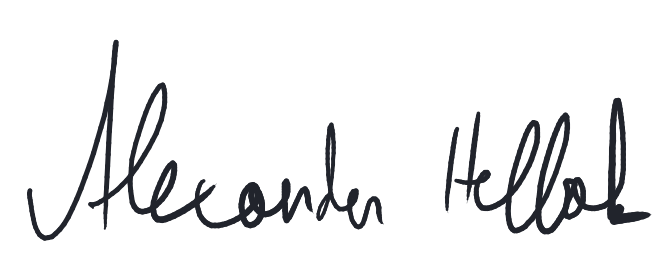
\includegraphics[scale=0.3]{alex_sign}
\end{minipage}

\begin{minipage}{0.3\textwidth}
	\vspace{-13.4cm}
	
\includegraphics[scale=1]{UnterschriftHugo}
\end{minipage}

\begin{minipage}{0.3\textwidth}
	\vspace{-7.4cm}
	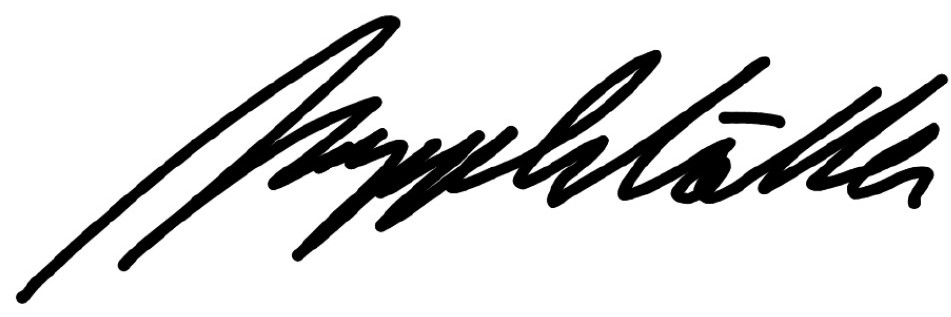
\includegraphics[scale=0.2]{max_sign}
\end{minipage}

\end{document}
